\subsection{Quality of Service Metrics} \label{sec:quality-of-service-metrics}

\begin{figure*}
  \centering
  \begin{subfigure}[b]{0.5\textwidth}
    \centering
    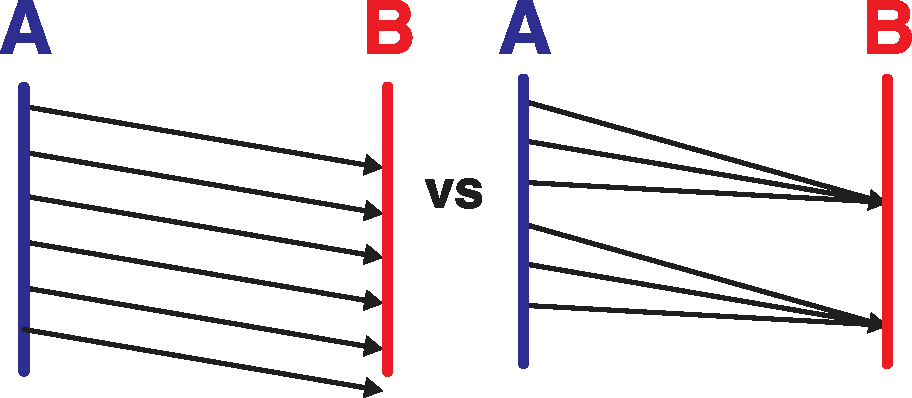
\includegraphics[width=\linewidth]{img/quality-of-service-metric-definitions/clumpiness.pdf}
    \caption{Clumpiness}
    \label{fig:quality-of-service-metric-definitions-clumpiness}
  \end{subfigure}%
  \begin{subfigure}[b]{0.5\textwidth}
    \centering
    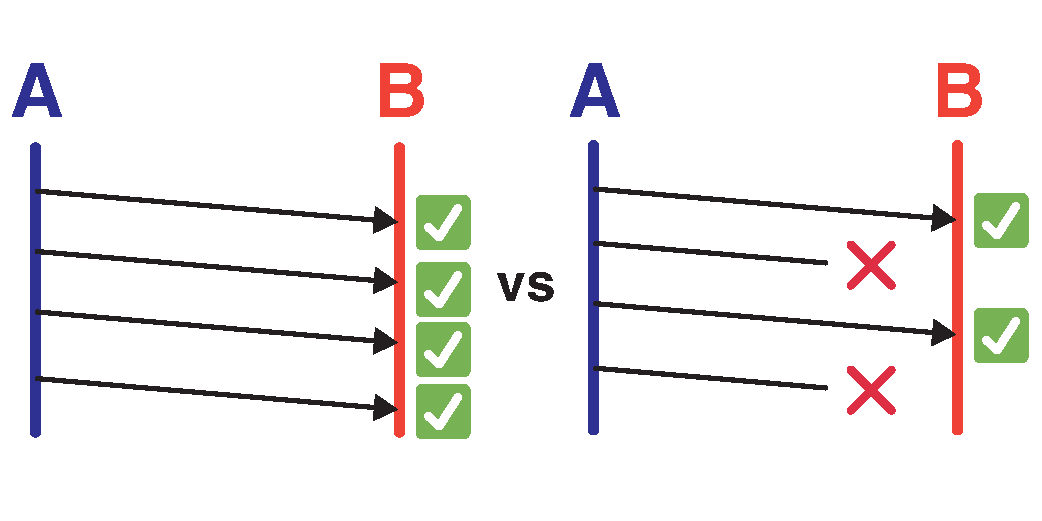
\includegraphics[width=\linewidth]{img/quality-of-service-metric-definitions/delivery-failure-rate.pdf}
    \caption{Delivery Failure Rate}
    \label{fig:quality-of-service-metric-definitions-delivery-failure-rate}
  \end{subfigure}
  \begin{subfigure}[b]{0.5\textwidth}
    \centering
    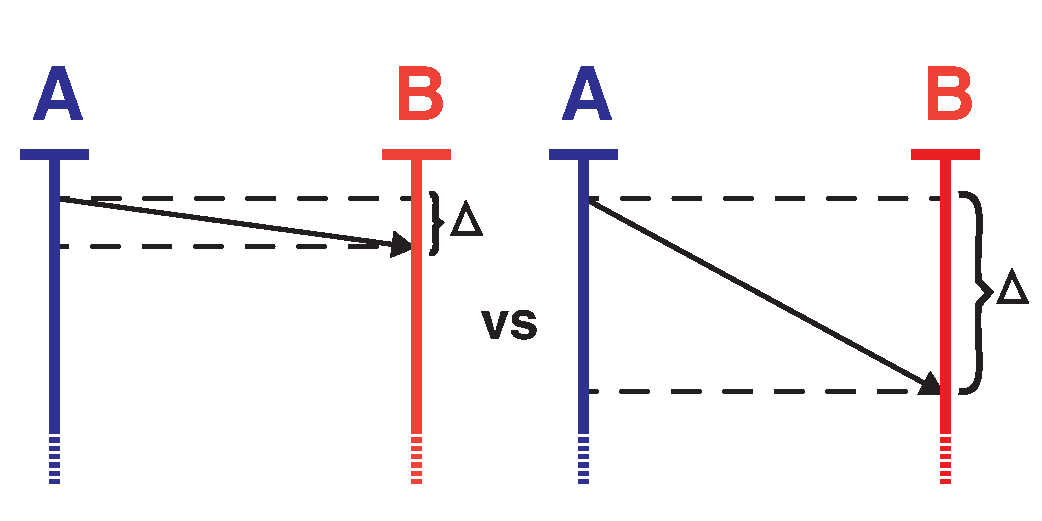
\includegraphics[width=\linewidth]{img/quality-of-service-metric-definitions/latency.pdf}
    \caption{Latency}
    \label{fig:quality-of-service-metric-definitions-latency}
  \end{subfigure}%
  \begin{subfigure}[b]{0.5\textwidth}
    \centering
    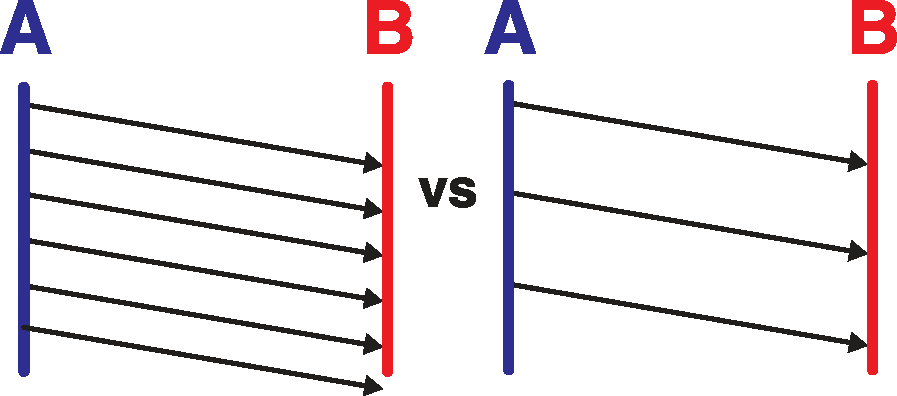
\includegraphics[width=\linewidth]{img/quality-of-service-metric-definitions/simstep-period.pdf}
    \caption{Simstep Period}
    \label{fig:quality-of-service-metric-definitions-simstep-period}
  \end{subfigure}%
  \caption{
  Quality of service metrics.
  Each illustration is a space-time diagram, with $A$ and $B$ representing independent processes.
  The vertical axis depicts the passage of time, from top to bottom.
  Solid black arrows represent message delivery.
  The left panel of each metric's diagram depicts a scenario with a lower (``better'') value for that metric compared to the right panel, which depicts a higher (``worse'') value for that metric.
  }
  \label{fig:quality-of-service-metric-definitions}
\end{figure*}


The best-effort communication model eschews effort to insulate computation from real-time message delivery dynamics.
Because these dynamics are difficult to predict \textit{a priori} and can bias computation, thorough, empirical runtime measurements are necessary to understand results of such computation.
To this end, we developed a suite of quality of service metrics.
Figure \ref{fig:quality-of-service-metric-definitions} provides space-time diagrams illustrating the metrics presented in this section.

For the purposes of these metrics, we assume that simulations proceed in an iterative fashion with alternating compute and communication phases.
For short, we refer to a single compute-communication cycle as a ``simstep.''
We derive formulas for metrics in terms of independent observations preceding and succeeding a ``snapshot'' window, during which the simulation and any associated best-effort communication proceeds unimpeded.
Snapshot observations are taken at one minute intervals over the course of each of our a replicate experiments.
The following section, \ref{sec:quality-of-service-experiments}, details the experimental apparatus used to generate quality of service metrics reported in this work.

\subsubsection{Simstep Period} \label{sec:simstep-period-metric}

We calculate the amount of wall-time elapsed per simulation update cycle (``Simstep Period'') during a snapshot window as
\begin{align*}
\frac{
  \mathrm{update\,count\,after} - \mathrm{update\,count\,before}
}{
  \mathrm{walltime\,after} - \mathrm{walltime\,before}
}.
\end{align*}
Figure \ref{fig:quality-of-service-metric-definitions-simstep-period} compares a scenario with low simstep period to a scenario with a higher simstep period.

\subsubsection{Simstep Latency} \label{sec:wall-time-latency-metric}

This metric reports the number of simulation iterations that elapse between message dispatch and message delivery.
Figure \ref{fig:quality-of-service-metric-definitions-latency} compares a scenario with low latency to a scenario with a higher latency.

To prevent interfering effects of imperfect clock synchronization between processes, we estimate one-way wall-time latency from a round-trip measure.
As part of our instrumentation, each simulation element maintains an independent zero-initialized ``touch counter'' for each neighbor simulation element it communicates with.
Dispatched messages are bundled with the current value touch counter associated with the target element.
Every message received sets the corresponding touch counter to $1 + \mathrm{bundled\,touch\,count}$.
In this manner, the touch counter increments by two for each successful round trip completed.
(Because simulation elements are arranged as a toroidal mesh in all experiments, interaction between simulation elements is always reciprocal.)

We therefore calculate one-way latency during a snapshot window as,
\begin{align*}
  \frac{
    \mathrm{update\,count\,after} - \mathrm{update\,count\,before}
  }{
    \min\Big( \mathrm{ touch\,count\,after } - \mathrm{ touch\,count\,before }, 1 \Big)
  }.
\end{align*}
Note that, in the case where no touches elapse, we bound our latency measure to snapshot duration.

%TODO reference @rodsan's derivation and proof

\subsubsection{Wall-time Latency} \label{sec:simulation-time-latency-metric}

Wall-time latency is closely related to simstep latency, simply denominating in elapsed real time instead of elapsed simulation steps.
To calculate wall-time latency we apply a conversion to simstep latency based on simstep period,
\begin{align*}
  \mathrm{simstep\,latency} \times \mathrm{simstep\,period}.
\end{align*}

This metric directly tells the real-time performance of message transmission.
Although it directly follows from the interaction between simstep period and wall-time latency, it complements simstep latency's convenient interpretation in terms of potential simulation mechanics (e.g., simulation elements tending to see data from two updates ago versus from ten).

In addition to simstep latency, Figure \ref{fig:quality-of-service-metric-definitions-latency} is also representative of wall-time latency --- simply interpreting the $y$ axis in terms of wall-time instead of elapsed simulation updates.

\subsubsection{Delivery Failure Rate} \label{sec:delivery-failure-rate-metric}

Delivery failure rate measures the fraction of messages sent that are dropped.
The only condition where messages are dropped is when a send buffer fills.
(Under the existing MPI-based implementation, messages that queue on the send buffer are guaranteed for delivery.)
So, we can calculate
\begin{align*}
  \frac{
    \mathrm{successful\,send\,count\,after} - \mathrm{successful\,send\,count\,before}
  }{
    \mathrm{attempted\,send\,count\,after} - \mathrm{attempted\,send\,count\,before}
  }.
\end{align*}

\subsubsection{Delivery Clumpiness} \label{sec:delivery-clumpiness-metric}

Delivery clumpiness quantifies the extent to which message arrival is consolidated to a subset of message pull attempts.
That is, the extent to which independently dispatched messages arrive in batches rather than as an even stream.

If messages all arrive in independent pull attempts, then clumpiness will be zero.
At the point where the pigeonhole principle applies (i.e., $\mathrm{num\,arriving\,messages} >= \mathrm{num\,pull\,attempts}$), clumpiness will also be zero so long as every pull attempt is laden.
If all messages arrive during a single pull attempt, then clumpiness will approach 1.

We formulate clumpiness as the compliment of steadiness.
(Reporting clumpiness provides a lower-is-better interpretation consistent with the rest of the quality of service metrics.)
Steadiness, in turn, stems from three component statistics,
\begin{align*}
\mathrm{num\,laden\,pulls\,elapsed} =& \mathrm{laden\,pull\,count\,after} \\
  &- \mathrm{laden\,pull\,count\,before} \\
\mathrm{num\,messages\,received} =& \mathrm{message\,count\,after} \\
  &- \mathrm{message\,count\,before} \\
\mathrm{num\,pulls\,attempted} =& \mathrm{pull\,attempt\,count\,after} \\
  &- \mathrm{pull\,attempt\,count\,before}
.
\end{align*}

Here, we refer to pull attempts that successfully retrieve a message as ``laden.''

We combine $\mathrm{num\,messages\,received}$ and $\mathrm{num\,pulls\,attempted}$ to derive,
\begin{align*}
  \mathrm{num\,opportunities\,for\,laden\,pulls} = \\
   \min\Big(\mathrm{num\,messages\,received}, \mathrm{num\,pulls\,attempted}\Big).
\end{align*}

Then, to calculate steadiness,
\begin{align*}
  \frac{
    \mathrm{num\,laden\,pulls\,elapsed}
  }{
    \mathrm{num\,opportunities\,for\,laden\,pulls}
  }.
\end{align*}

Delivery clumpiness follows as $1 - \mathrm{steadiness}$.
Figure \ref{fig:quality-of-service-metric-definitions-clumpiness} compares a scenario with low clumpiness to a scenario with higher clumpiness.
